\documentclass[a4paper]{article}
\usepackage{comment}
\usepackage[utf8]{inputenc}
\usepackage[spanish]{babel}
\usepackage{amsmath}
\usepackage{amssymb}
\usepackage{graphicx}
\usepackage[labelfont=bf, font=small,it]{caption}
\usepackage{todonotes}
\usepackage{hyperref}
\usepackage{geometry} % Page layout


\usepackage{caratulaMetNum}

\begin{document}

\setlength{\parskip}{3mm}
\setlength{\parindent}{7mm}

	\fecha{\today}
	\materia{Introducción al Procesamiento Digital de Imágenes}
	\titulo{Práctica 4 bis}
    \subtitulo{DFT}

	\integrante{Pazos Méndez, Nicolás Javier}{709/15}{npazosmendez@gmail.com}
	\integrante{Balbi, Pablo Luis}{707/15}{pablo.l.balbi@gmail.com}

	% \palabraClave{equalisation}
 %   	\palabraClave{HSI}
	% \palabraClave{images}
	% \palabraClave{cheese}

	% \abstracto{\hspace{5mm}Un método automático para particionar un histograma para aplicar el algoritmo de AEPHE.}

	\maketitle

\tableofcontents
\pagebreak

\section{Ejercicio 1}
\begin{center}

	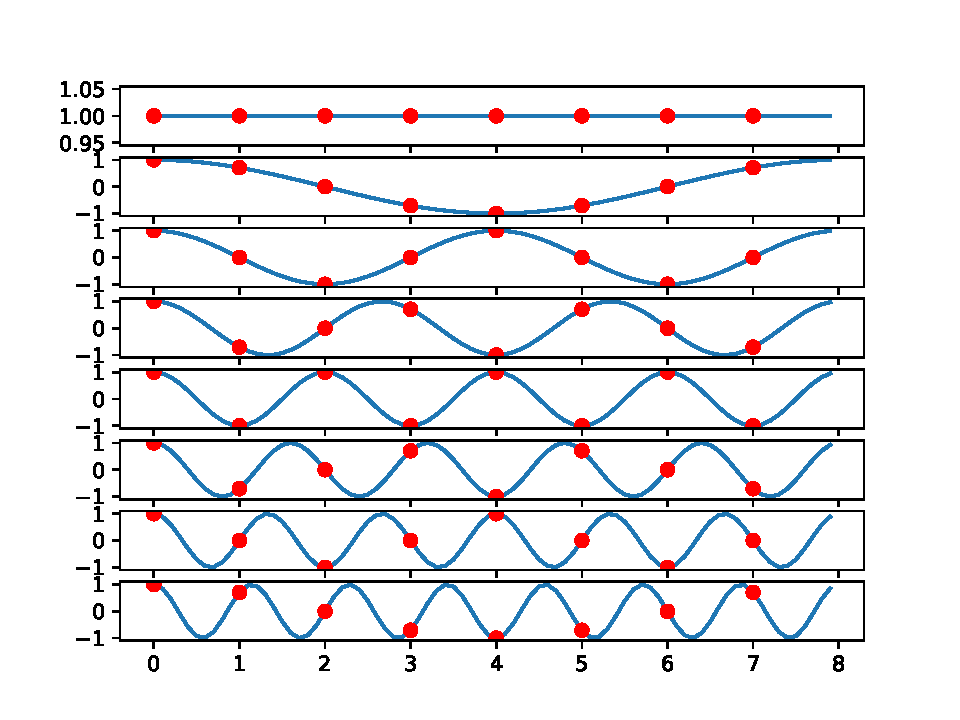
\includegraphics[scale=0.7]{imgs/1a.pdf}
	\captionof{figure}{Bases de Fourier para 8 dimensiones en 1-D}

	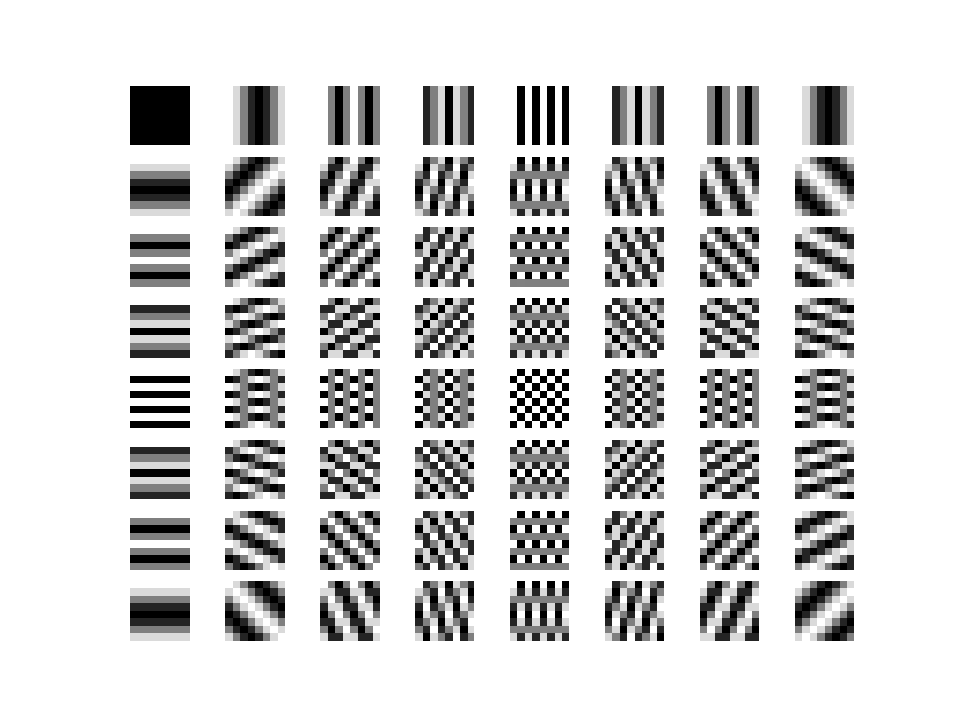
\includegraphics[scale=0.7]{imgs/1b.pdf}
	\captionof{figure}{Bases de Fourier para 8 dimensiones en 2-D}
\end{center}

\section{Ejercicio 2}

\begin{center}
	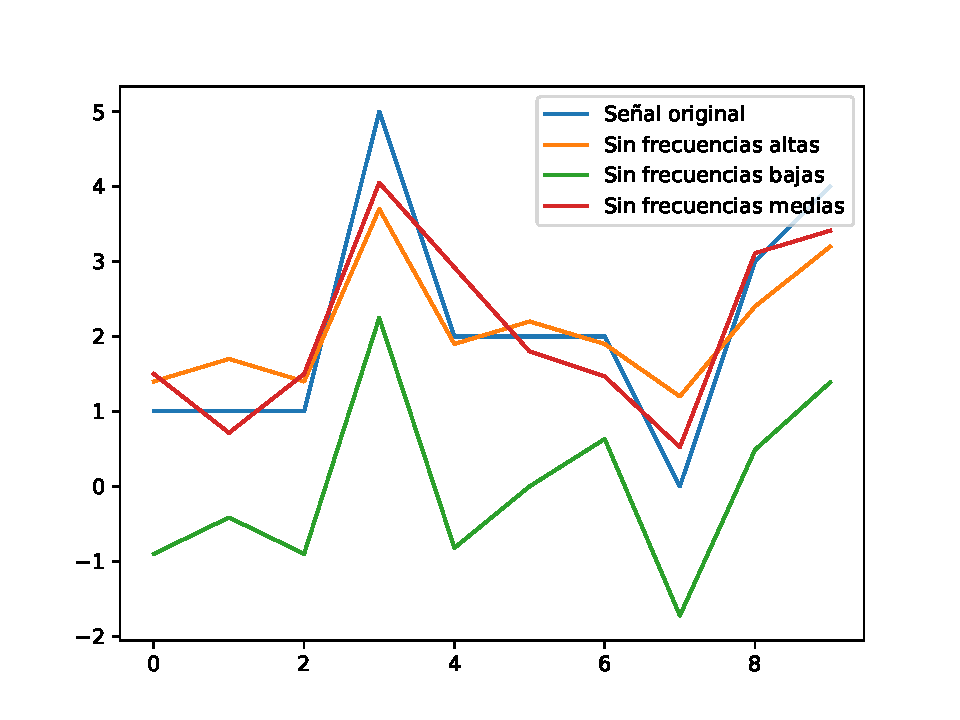
\includegraphics[scale=0.7]{imgs/2.pdf}
\end{center}

Puede verse como al perder las frecuencias bajas, la señal pierde información general pero conserva los detalles; se separa de la señal original, pero tiene los mismos picos. Al perder las frecuencias altas pasa exactamente lo contrario, y al conservar las medias se llega a un equilibrio.

\section{Ejercicio 3}

\begin{center}

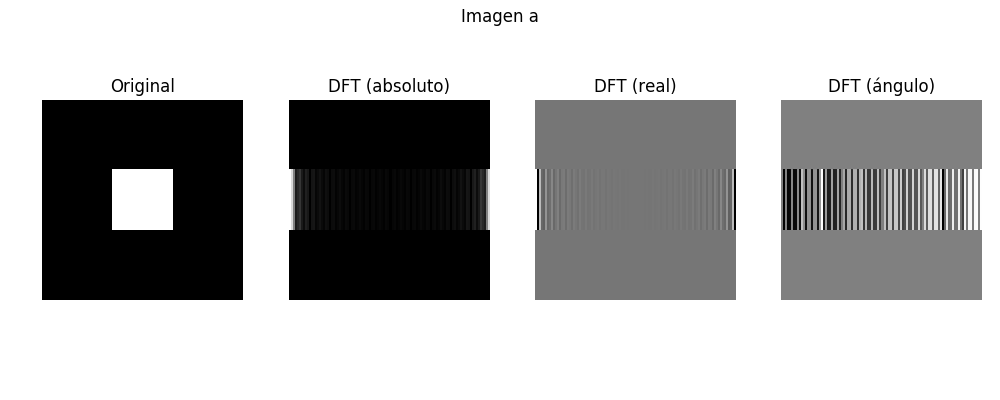
\includegraphics[scale=0.4]{imgs/3-a.png}

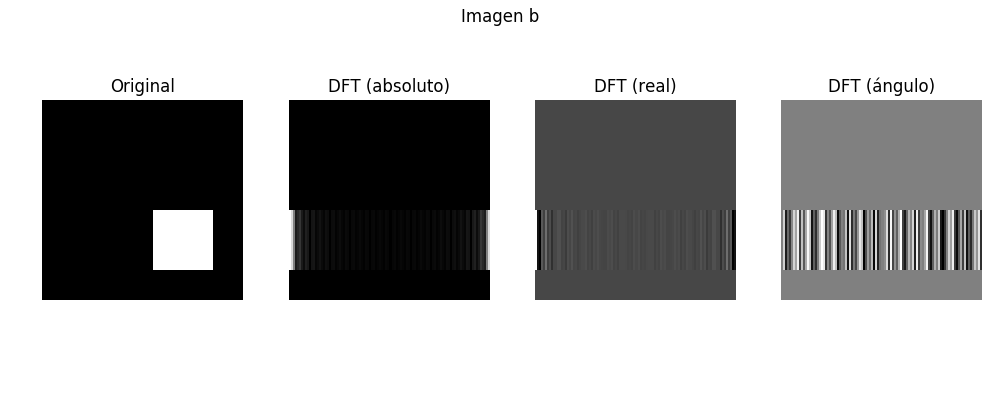
\includegraphics[scale=0.4]{imgs/3-b.png}

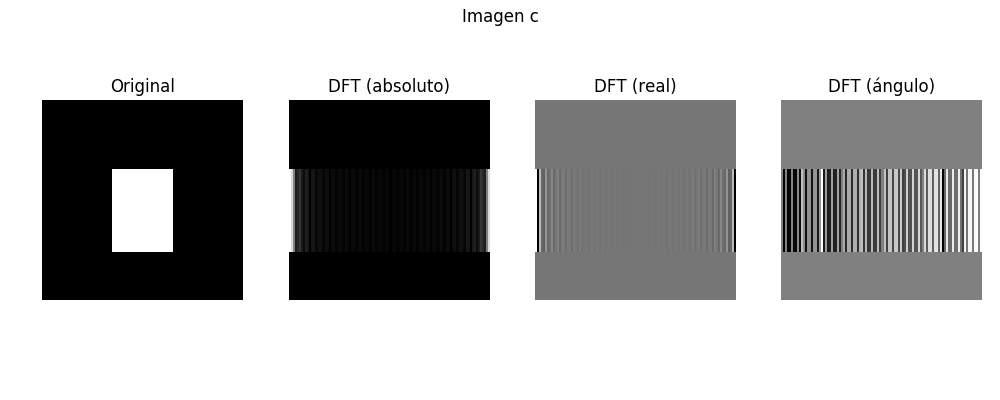
\includegraphics[scale=0.4]{imgs/3-c.png}

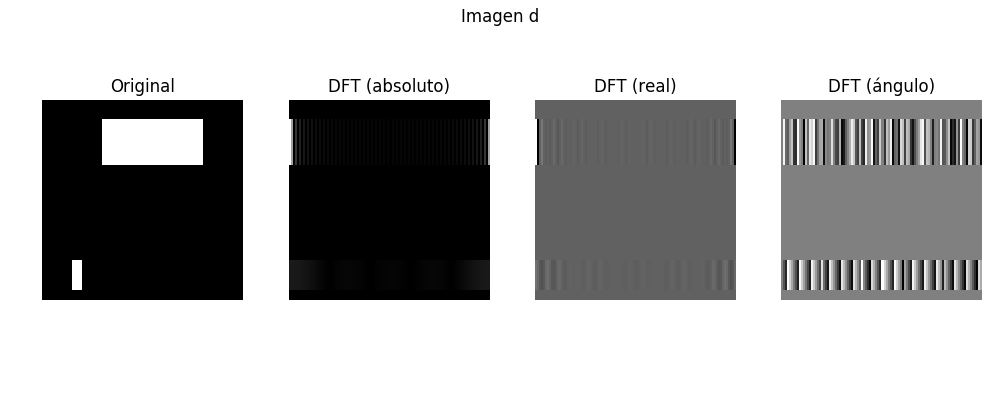
\includegraphics[scale=0.4]{imgs/3-d.png}

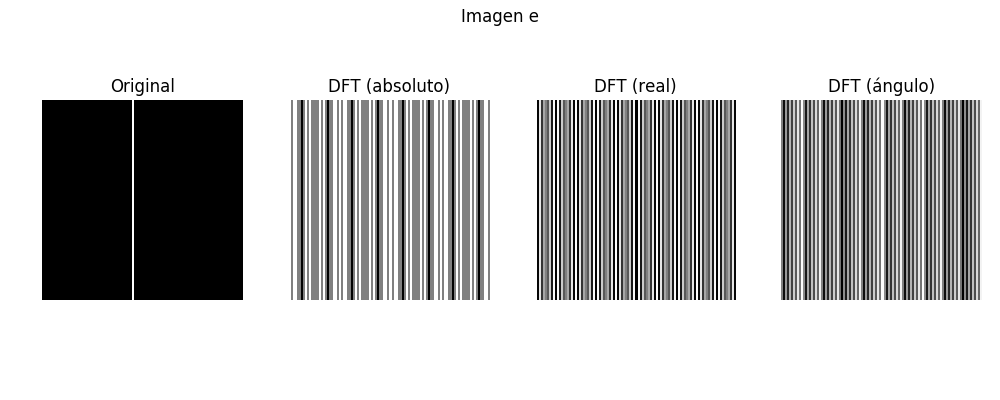
\includegraphics[scale=0.4]{imgs/3-e.png}

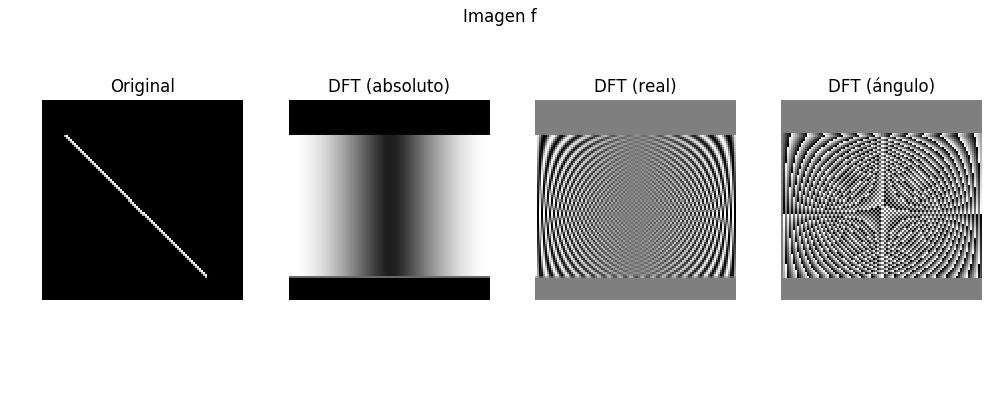
\includegraphics[scale=0.4]{imgs/3-f.png}

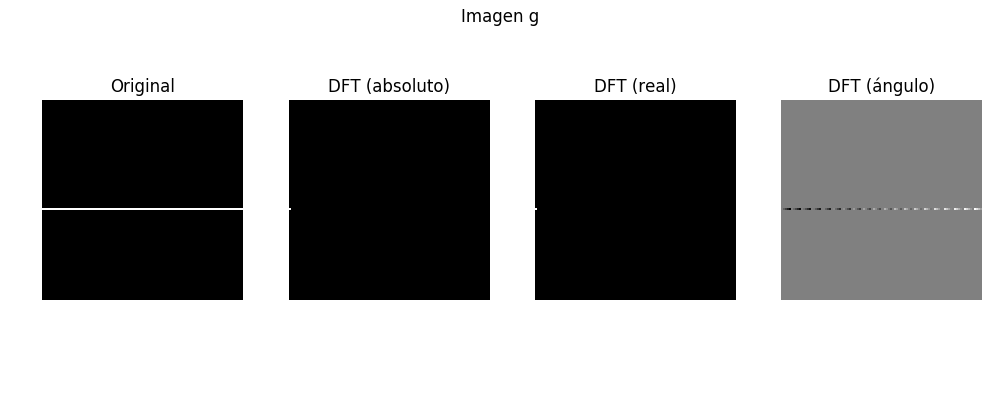
\includegraphics[scale=0.4]{imgs/3-g.png}

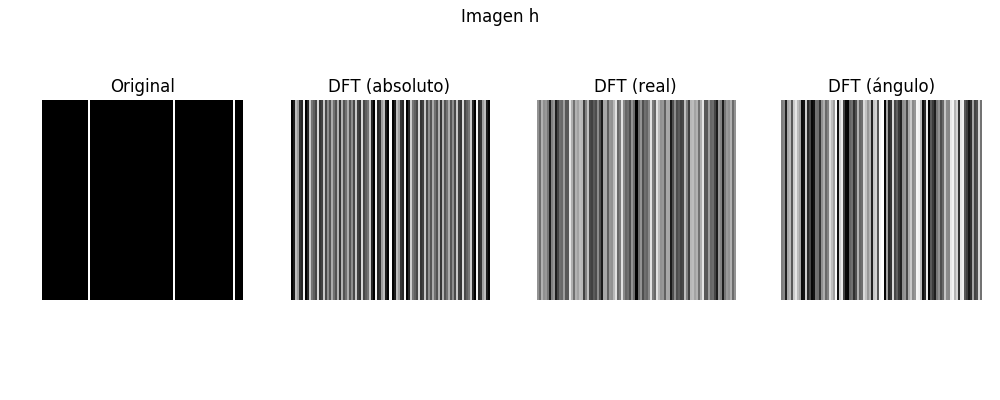
\includegraphics[scale=0.4]{imgs/3-h.png}

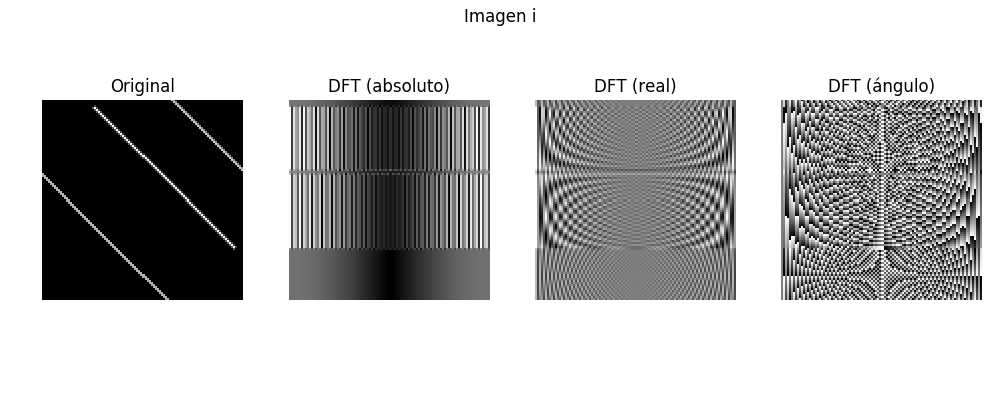
\includegraphics[scale=0.4]{imgs/3-i.png}

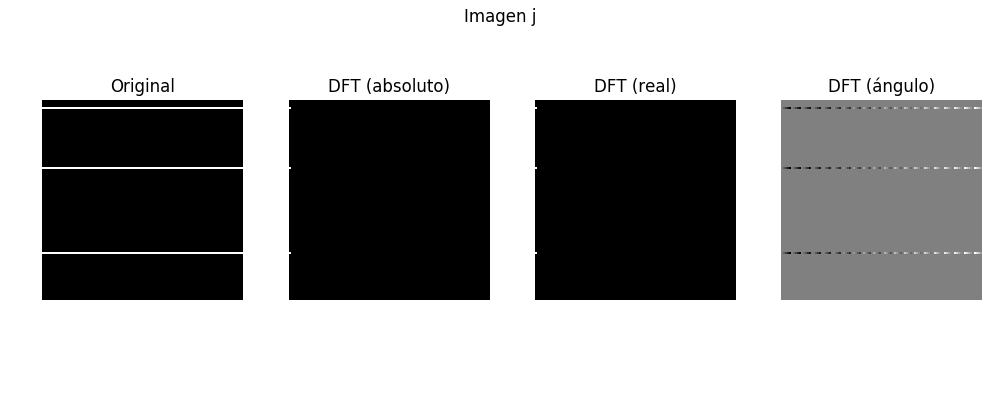
\includegraphics[scale=0.4]{imgs/3-j.png}
\end{center}

\section{Ejercicio 4}

Combinaremos las siguientes dos imágenes:

\begin{center}

	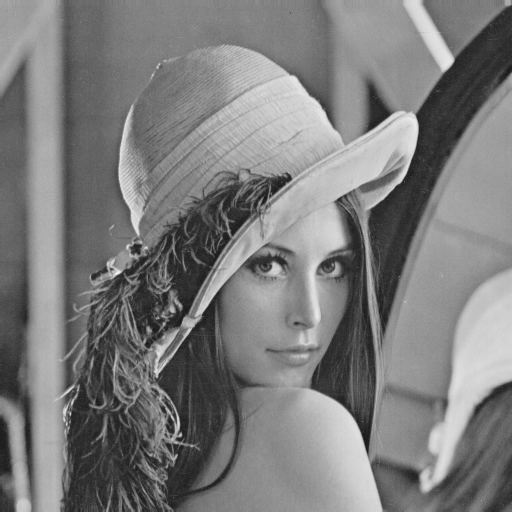
\includegraphics[scale=0.3]{imgs/lena.png}
	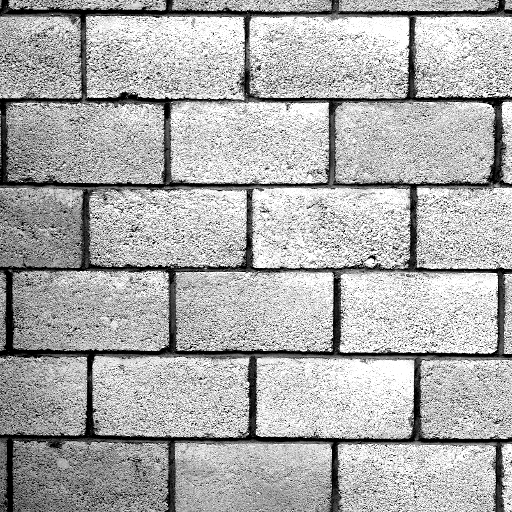
\includegraphics[scale=0.3]{imgs/ladrillos.png}
\end{center}

\begin{center}

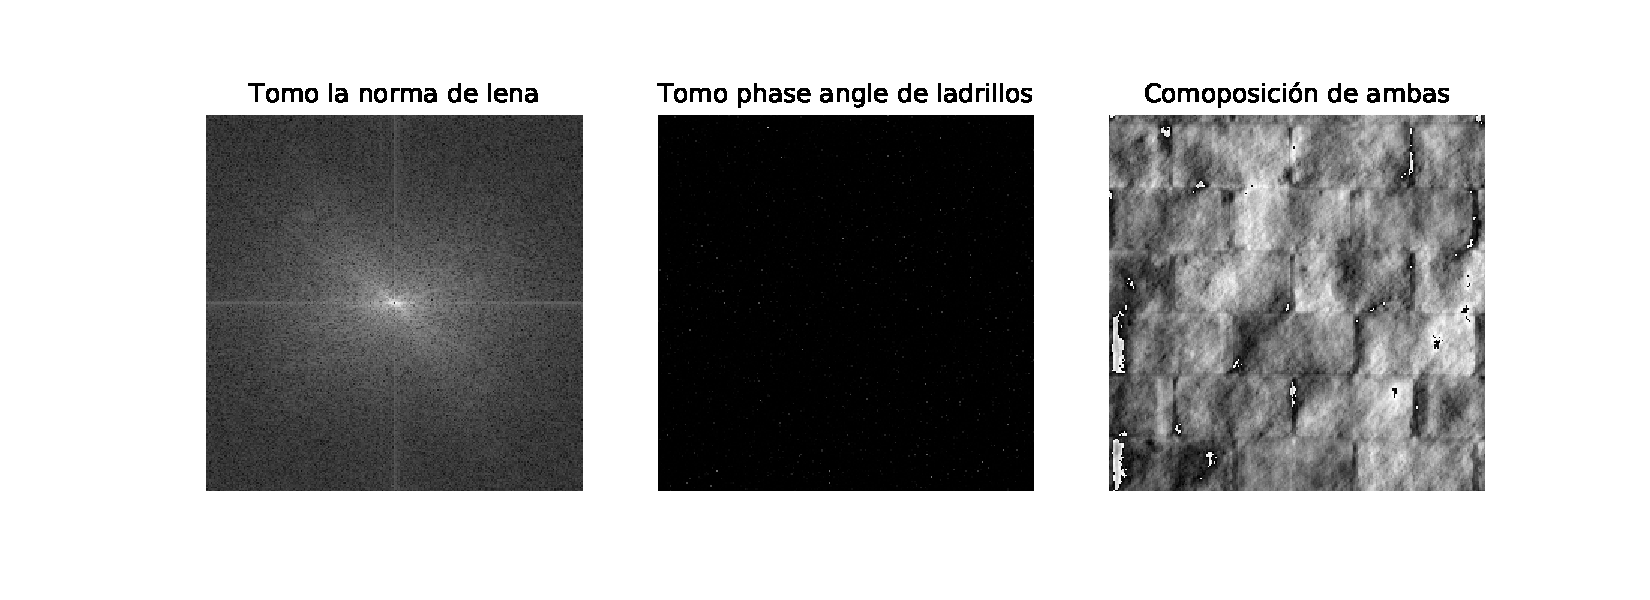
\includegraphics[scale=0.6]{imgs/4a.pdf}

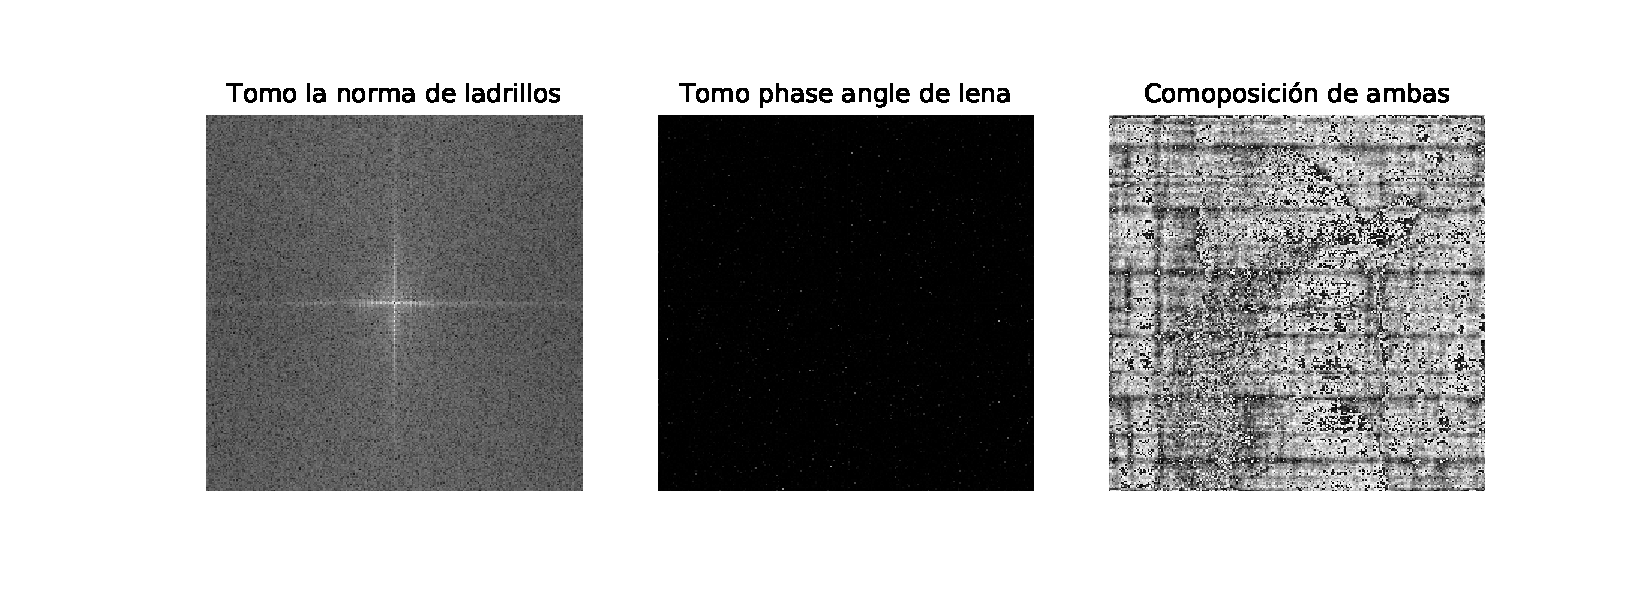
\includegraphics[scale=0.6]{imgs/4b.pdf}
\end{center}

% \section{Ejercicio 5}
\section{Ejercicio 6}
\begin{center}

	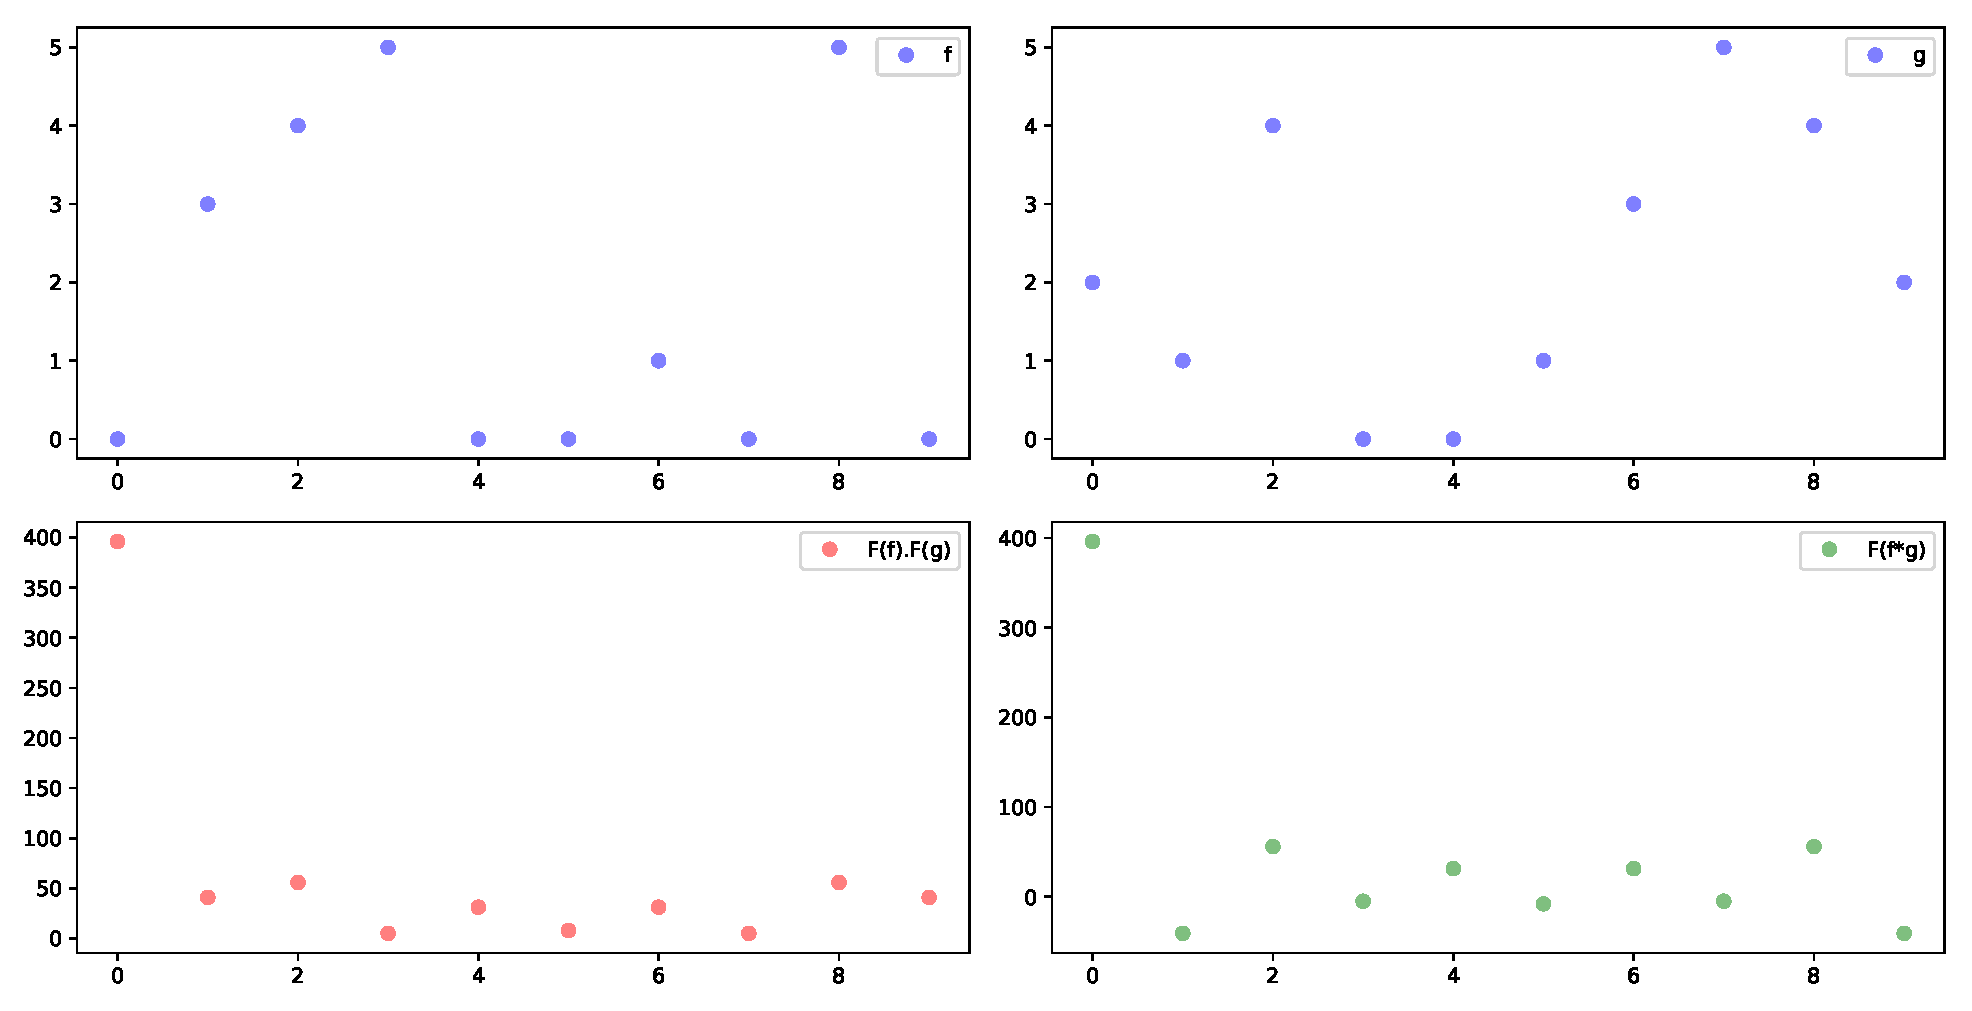
\includegraphics[scale=0.5]{imgs/6.pdf}
\end{center}



\end{document}
